\chapter{Continuous Random Variables}

The probability models we used earlier were discrete. Starting from this chapter, we will discuss some non-discrete probability models.

Suppose a postal package is to be delivered to you between noon and 1:00 pm. You have to leave home between 12:30 to 12:45 pm.

What is the probability you miss the delivery?

\section{Uniform Random Variable}
This question is quite simple, and we can immediately see that the answer is \(\frac{15}{60}\). However, how can we define a probability model here?

\begin{definition}[Uniform Random Variable]
    A uniform random variable \(T\) over interval \([0, 1]\) satisfies 
    \[
        \mathbb{P}(T \leq t) = \begin{dcases}
            0, &\text{ if } t \leq 0 ,\\
            t, &\text{ if } 0 < t \leq 1 ,\\
            1, &\text{ if } 1 < t.
        \end{dcases}
    \]
\end{definition}

Based on the above definition, we can calculate the following: 

\(
\begin{aligned}
    \mathbb{P}(T > \dfrac{1}{2}) &= 1 - \mathbb{P}(T \leq \dfrac{1}{2}) = 1 - \dfrac{1}{2} = \dfrac{1}{2} \\
    \mathbb{P}(T > \dfrac{3}{4}) &= 1 - \mathbb{P}(T \leq \dfrac{3}{4}) = 1 - \dfrac{3}{4} = \dfrac{1}{4} \\
    \mathbb{P}(\dfrac{1}{2} < T \leq \dfrac{3}{4}) &= \mathbb{P}(T > \dfrac{1}{2}) - \mathbb{P}(T > \dfrac{3}{4}) = \dfrac{1}{2} - \dfrac{1}{4} = \dfrac{1}{4}
\end{aligned}
\) 

\begin{eg}[Continuous Random Variables and Zero Probability for Points]~ 
    Consider a Uniform(\([0, 1]\)) random variable \(T\). 

    1. \(\mathbb{P}(T \leq 0.3) = 0.3\) 

    2. \(\mathbb{P}(T = 0.3) = 0\)
        
    Assume that \(\mathbb{P}(T = 0.3) = \varepsilon > 0\), \(\mathbb{P}(T \leq 0.3 - \frac{\varepsilon}{4}) = 0.3 - \frac{\varepsilon}{4}\), \(\mathbb{P}(T \leq 0.3 + \frac{\varepsilon}{4}) = 0.3 + \frac{\varepsilon}{4}\)

    Above gives \(\mathbb{P}(0.3 - \frac{\varepsilon}{4} < T < 0.3 + \frac{\varepsilon}{4}) = \mathbb{P}(T \leq 0.3 + \frac{\varepsilon}{4}) - \mathbb{P}(T \leq 0.3 - \frac{\varepsilon}{4}) = \frac{\varepsilon}{2}\) 

    However, for \(\mathbb{P}(T = 0.3) \subseteq \mathbb{P}(0.3 - \frac{\varepsilon}{4} < T < 0.3 + \frac{\varepsilon}{4})\), we have \(\varepsilon < \frac{\varepsilon}{2}\), which by contradiction shows that \(\mathbb{P}(T = 0.3) = 0\)

    3. \(\mathbb{P}(T < 0.3) = \mathbb{P}(T \leq 0.3) - \mathbb{P}(T = 0.3) = 0.3\)
\end{eg}

Above shows that the probability mass function (PMF) does not make much sense because \(\mathbb{P}(T = t) = 0\) for every \(t\).

\section{Cumulative Distribution Function (CDF)}
The Cumulative Distribution Function works for both discrete and continuous probabilities.
\begin{definition}[Cumulative Distribution Function (CDF)]
  The cumulative distribution function (CDF) \(F\) of a random variable \(X\) is:
  \[
    F(x) = \mathbb{P}(X \leq x)
  \]
\end{definition}

Every CDF \(F:\mathbb{R} \to [0, 1]\) must satisfy the following properties:

1. \(F\) is monotonically increasing: \(x \leq y \Longrightarrow F(x) \leq F(y)\)

2. \(\lim_{n \to -\infty} F(x) = 0\) 

3. \(\lim_{n \to +\infty} F(x) = 1\) 

\begin{eg}
    Find the CDF of a Geometric(\(p = \frac{1}{2}\)) random variable.

    \textbf{Solution:} 
    \[
        F(k) = \mathbb{P}[X \leq k] = 1 - \mathbb{P}[X > k] = 1 - (1 - p)^k
    \]
\end{eg}

By observation, we see that the CDF of a Uniform random variable over interval \([0, 1]\) is 
\[
    \mathbb{P}(X \leq x) = \begin{dcases}
        0, &\text{ if } x \leq 0 ,\\
        x, &\text{ if } 0 < x \leq 1 ,\\
        1, &\text{ if } 1 < x.
    \end{dcases}
\]

\subsection{Probability Density Function (PDF)}
\begin{definition}[Probability Density Function (PDF)]
    For a continuous random variable \(X\), we define its probability density function (PDF) \(f\) as the derivative of its CDF:
    \[
        f(X) \coloneqq \lim_{\delta \to 0} \dfrac{\mathbb{P}(x \leq X \leq x + \delta)}{\delta}= \lim_{\delta \to 0} \dfrac{F(x + \delta) - F(x)}{\delta} = \frac{\mathrm{d}F(x)}{\mathrm{d}x}  
    \]

    \begin{remark}
        PDF is not probability, it is the rate of probability. 
    \end{remark}
\end{definition}

For a small \(\delta > 0\), we know \(F(x + \delta) - F(x) \approx f(x)\delta\) and so for small \(\delta \), 
\[
    \mathbb{P}(x \leq X \leq x + \delta) \approx f(x)\delta
\]

For example, 
\[
    F(x) = \begin{dcases}
        0, &\text{ if } x < 0 ,\\
        x, &\text{ if } 0 \leq  x \leq 1 ,\\
        1, &\text{ if } 1 < x.
    \end{dcases}
    \quad\Longrightarrow\quad 
    f(x) = \begin{dcases}
        0, &\text{ if } x < 0 ,\\
        1, &\text{ if } 0 \leq x \leq 1 ,\\
        0, &\text{ if } 1 < x.
    \end{dcases}
\]

\begin{eg}
    The CDF of random variable \(X\) is \(F(x) = \begin{dcases}
        1 - \frac{1}{x^2}, &\text{ if } x > 1 \\
        0, &\text{ if } x \leq 1 
    \end{dcases}\). 
    
    Find the PDF of \(X\).

    \textbf{Solution:} 
    First, we need to verify whether it is a valid CDF. Since it satisfies the three properties, we can then determine the PDF of \(X\).
    \[
        f(x) = \frac{\mathrm{d}F(x)}{\mathrm{d}x} = \begin{dcases}
            \dfrac{2}{x^3}, &\text{ if } x > 1 \\
            0 , &\text{ if } x \leq 1 
        \end{dcases}
    \]

\end{eg}


\begin{minipage}{0.5\textwidth}
    \centering
    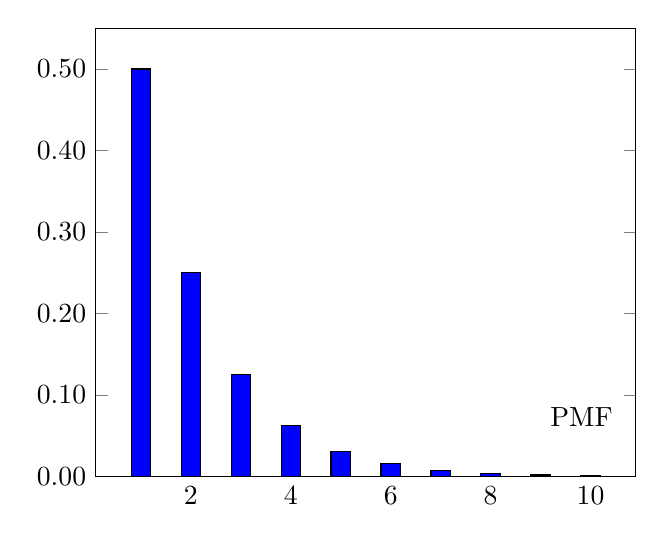
\begin{tikzpicture}
        \begin{axis}[
            ymin=0,
            ymax=0.55,
            xtick={0,2,...,10},
            ytick={0,0.1,...,0.5},
            samples at={1,...,10},
            xtick style={draw=none},
              yticklabel style={
                  /pgf/number format/fixed,
                  /pgf/number format/fixed zerofill,
                  /pgf/number format/precision=2,
            },   
            domain=1:10,
            samples=10,
        ]
        % Define p, probability of success
        \pgfmathsetmacro{\p}{0.5}
        
        % Plot the PMF of the geometric distribution
        \addplot [
          ybar=0pt,
          bar width=7pt,
          fill=blue,
          mark=none,
      ] {(\p*(1-\p)^(x-1))};
      % Add "discrete CDF" label
      \node[anchor=south west] at (axis cs:9,0.05) {PMF};
        \end{axis}
    \end{tikzpicture}
\end{minipage}
\begin{minipage}{0.5\textwidth}
    \centering
    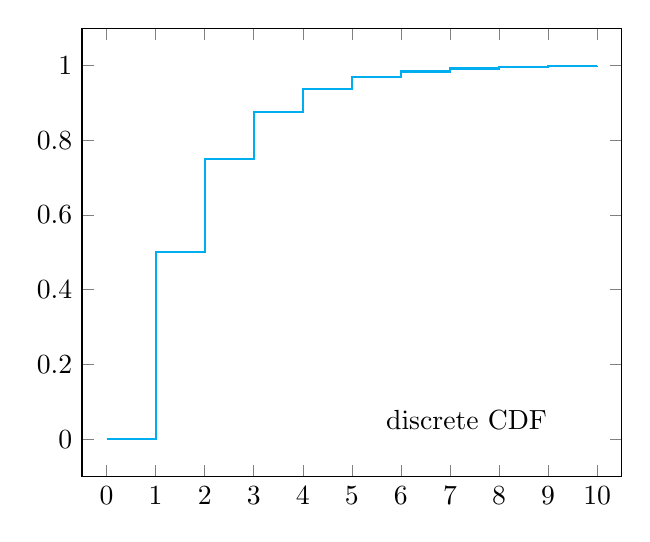
\begin{tikzpicture}
    \begin{axis}[
        axis lines=box,
        xtick={0,1,...,10},
        ytick={0,0.2,...,1},
        ymin=-0.1, ymax=1.1,
        xmin=-0.5, xmax=10.5,
        every axis x label/.style={at={(ticklabel* cs:1)}, anchor=north},
        every axis y label/.style={at={(ticklabel* cs:1)}, anchor=east},
    ]
        % Plot the stepwise CDF
        \addplot[
            thick,
            cyan,
            const plot
        ] coordinates {
            (0, 0)
            (1, 0.5)
            (2, 0.75)
            (3, 0.875)
            (4, 0.9375)
            (5, 0.96875)
            (6, 0.984375)
            (7, 0.9921875)
            (8, 0.99609375)
            (9, 0.998046875)
            (10, 0.999023437)
        };

        % Add "discrete CDF" label
        \node[anchor=south west] at (axis cs:5.5,0) {discrete CDF};
    \end{axis}
\end{tikzpicture}
\end{minipage}

\begin{minipage}{0.5\textwidth}
    \centering
    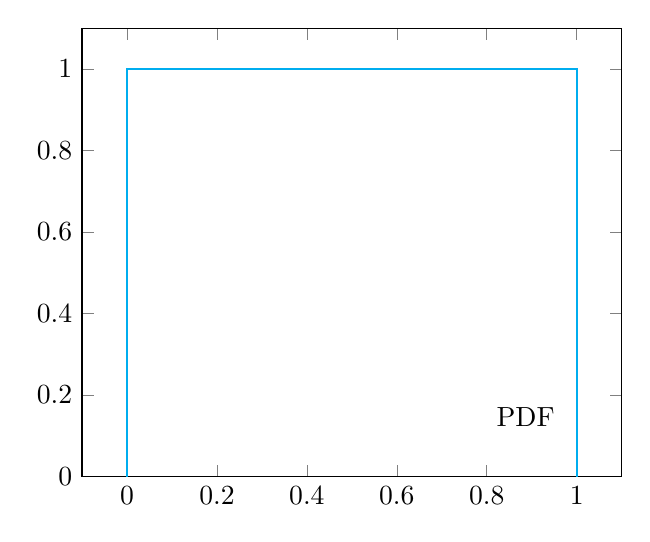
\begin{tikzpicture}
        \begin{axis}[
            axis lines=box,
            xtick={0,0.1,...,1.0},
            ytick={0,0.2,...,1.0},
            xmin=-0.1, xmax=1.1,
            ymin=0.0, ymax=1.1,
            xtick={0,0.2,...,1.0},
            ytick={0,0.2,...,1.0},
            samples at={0.0,...,1.0},
        ]
            % Plot the stepwise CDF
            \addplot[
                thick,
                cyan,
                const plot
            ] coordinates {
                (0.0, 0.0)
                (0.0, 1.0)
                (0.1, 1.0)
                (0.2, 1.0)
                (0.3, 1.0)
                (0.4, 1.0)
                (0.5, 1.0)
                (0.6, 1.0)
                (0.7, 1.0)
                (0.8, 1.0)
                (0.9, 1.0)
                (1.0, 0.0)
            };
            % Add "discrete CDF" label
            \node[anchor=south west] at (axis cs:0.8,0.1) {PDF};
        \end{axis}
    \end{tikzpicture}
\end{minipage}
\begin{minipage}{0.5\textwidth}
    \centering
    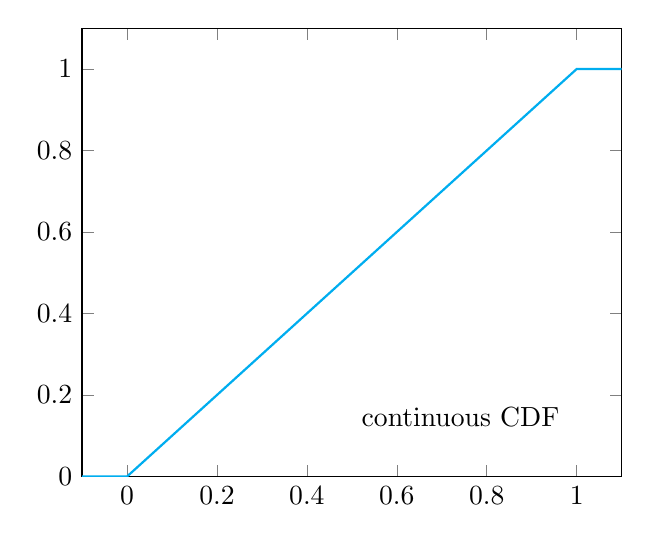
\begin{tikzpicture}
        \begin{axis}[
            axis lines=box,
            xtick={0,0.1,...,1.0},
            ytick={0,0.2,...,1.0},
            xmin=-0.1, xmax=1.1,
            ymin=0.0, ymax=1.1,
            xtick={0,0.2,...,1.0},
            ytick={0,0.2,...,1.0},
            samples at={0.0,...,1.0},
        ]
            % Plot the stepwise CDF
            \addplot[
                thick,
                cyan,
            ] coordinates {
                (-0.1, 0.0)
                (0.0, 0.0)
                (1.0, 1.0)
                (1.1, 1.0)
            };
            % Add "discrete CDF" label
            \node[anchor=south west] at (axis cs:0.5,0.1) {continuous CDF};
        \end{axis}
    \end{tikzpicture}
\end{minipage}
